% %%%%%%%%%%%%%%%%%%%%%%%%%%%%%%%%%%%%%%%%%%%%%%%%%%%%%%%%%%%%%%%%%%%%%
% %% State-of-the-Art %%
% ExTensor
% %%%%%%%%%%%%%%%%%%%%%%%%%%%%%%%%%%%%%%%%%%%%%%%%%%%%%%%%%%%%%%%%%%%%%

\subsection{ExTensor}
\label{sec:soa:extensor}

The authors created ExTensor~\cite{Hegde2019_ExTensor} as a general purpose sparse tensor algebra accelerator (including SpMSpM). It is an \algo{OP} accelerator but due to its support for three levels of fixed \emph{tiling} of the inputs, it optimizes the \emph{intersection} search between non-zero elements or \emph{tiles}\footnote{Tensauraus~\cite{Srivastava2020_Tensaurus} is another accelerator designed for tensors, but their focus is on SpMM.}. By doing the \emph{intersections} ahead of time, at different levels of the memory hierarchy (which correspond to the \emph{tile} levels), ExTensor is able to efficiently eliminate \emph{ineffectual operations}, thus addressing the main issue in \algo{IP} or complex \emph{tiling} algorithms. Indeed, the input matrices would typically be stored in an \emph{(UOP, UOP, UOP, CP}) format, corresponding to three levels of \emph{tiling}.
ExTensor is designed with a flexible architecture composed of different bricks (see Figure~\ref{fig:soa:extensor}). To simply aid in the understanding, the interactions between the bricks are described using function calls:
\begin{itemize}
    \item The \emph{Scanner} is a storage unit that delivers a stream of coordinates in increasing order, fetching them from memory. The coordinates are delivered through the \emph{Iterate()} operation call.
    \item The \emph{Intersect} is a hardware block that co-iterates over several \emph{Scanners} in parallel and compares the coordinate streams. This unit performs the \emph{intersection} search required by \algo{IP} type algorithms, delivering a single stream with the matching coordinates, which are the coordinates of non-zero \emph{partial sums}. To optimise the \emph{intersection} step, it is possible to skip a range of coordinates in a stream depending on the current coordinate of another stream. Thus, the \emph{Intersect} sends skip messages with \emph{SkipTo()} operations to the other \emph{Scanners}.
    \item The \emph{Coordinator} is a hardware unit that includes \emph{Scanners} and \emph{Intersect} units, and manages the input and output data depending on the current processed \emph{tile}, as shown in Figure~\ref{fig:soa:extensor}. Data and \emph{metadata} are respectively stored in storage units and \emph{Scanners}, while a \emph{Sequencer} manages the \emph{Iterate()} calls so that the \emph{Intersect} brick delivers the stream of effective coordinates. In addition, in the \emph{Tile Coord} brick, the offsets of the \emph{tile} are added back, so the output of the \emph{Coordinator} is in absolute coordinates.
\end{itemize}

These bricks can be placed at different positions in a memory hierarchy, depending on the \emph{tiling} and selected hardware. Thus, the \emph{Coordinator} is able to intersect at coarse-granularity with output data being \emph{metadata} of the next \emph{tile}, skipping an entire \emph{tile} when appropriate, with low computation cost, and also at fine-granularity when output data are the non-zero elements that need to be multiplied.

ExTensor is designed with three levels of \emph{tiling} that each have  either input or output sequentiality. First, a \emph{Sequencer} plus \emph{Scanners} block~\ding{192} is placed close to the main memory to determine which \emph{tiles} to send to the next storage, the \emph{Last Level Buffer} (\emph{LLB}). Then, for each \emph{tile}, a \emph{Coordinator}~\ding{193} in the \emph{LLB} intersects the next level \emph{tiles}, which are sent to several \emph{PEs} that will process in parallel. Finally, in each \emph{PE}, a \emph{Coordinator}~\ding{194} intersects the non-zero elements of the computed \emph{tile} and sends them to the arithmetic unit of the \emph{PE} for multiplication.

In addition to these bricks which are the main contributions, ExTensor still needs to perform the \emph{merge} phase, including the \emph{reduction} of the \emph{POs} which are stored in \emph{CP$^{2}$} format. The \emph{Partial Output Buffer} (\emph{POB}), is managed by \emph{tiles}, and the content of the \emph{tile} is stored on-chip using a Content Addressable Memory (CAM) for quick access, enabling \emph{reductions} to be performed. On overflow, the \emph{tiles} are flushed to main memory. To benefit from ExTensor's support for \emph{tiling}, the input matrices need preprocessing, making it difficult to directly compare performance with other accelerators.

\begin{figure}
    \centering
    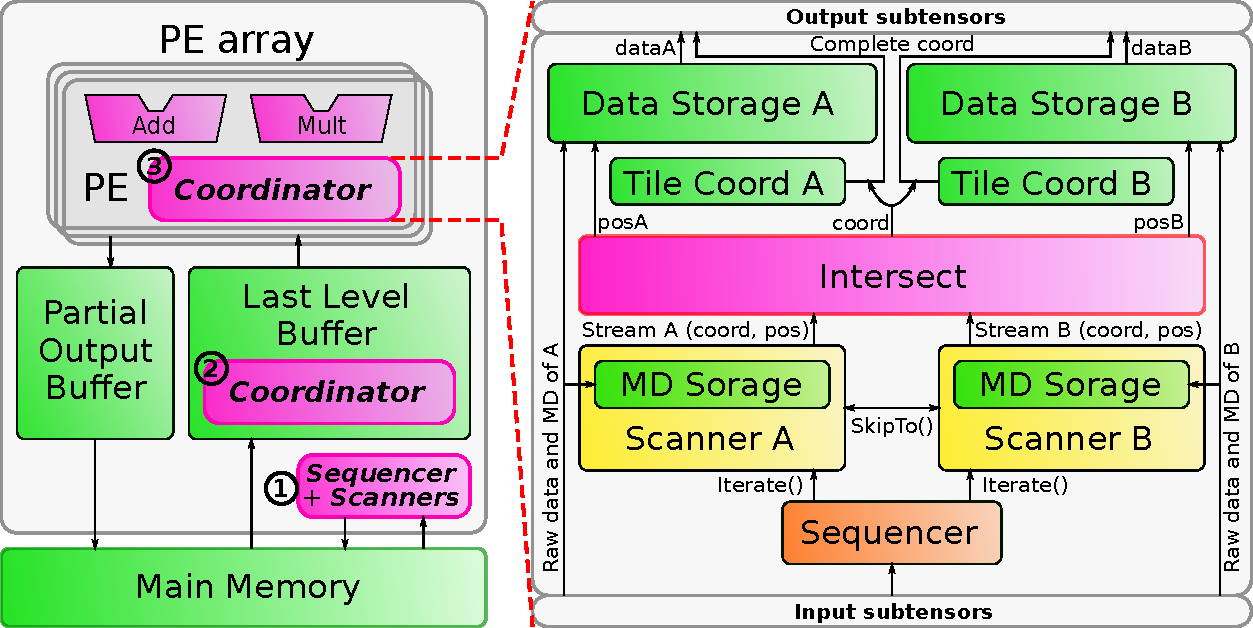
\includegraphics[width=0.6\linewidth]{Chapter_SoA/Figures/PDF/ExTensor.pdf}
    \caption{Architecture of ExTensor}
    \label{fig:soa:extensor}
\end{figure}